\documentclass[11pt]{article}
\usepackage[margin=1in]{geometry}
\usepackage{booktabs}
\usepackage{longtable}
\usepackage{array}
\usepackage{tabularx}
\usepackage{hyperref}
\usepackage{graphicx}
\graphicspath{{../}{../outputs/pc_algorithm/figures/}}
\usepackage{float}
\usepackage{pdflscape}
\usepackage{caption}
\usepackage{subcaption}
\usepackage{siunitx}
\usepackage{amsmath}
\usepackage{amssymb}

\title{PC Algorithm Results Report}
\author{ENLA Pipeline}
\date{\today}

\begin{document}
\maketitle

\section{Overview}
This report documents the causal discovery analyses performed with the Peter--Clark (PC) algorithm within the ENLA pipeline. The goal is to recover directed causal structures among questionnaire indicators and key academic outcomes:
\begin{itemize}
  \item socioemotional learning composite (\texttt{socioemotional\_learning})
  \item academic language performance (\texttt{academic\_lang})
  \item academic mathematics performance (\texttt{academic\_math})
\end{itemize}
All experiments rely on the preprocessed dataset generated by \texttt{pipeline/02\_preprocess.R} and are executed via \texttt{pipeline/05\_pc\_algorithm.R}.

\section{Methodology}
\subsection{Data Preparation}
We use the preprocessed object at \texttt{outputs/preprocessed/enla\_preprocessed.rds}. The \texttt{analysis} component contains harmonized performance indicators and weights; the \texttt{raw} component exposes the questionnaire microdata. We select the student questionnaire (\texttt{PC\_QUESTIONNAIRE=estudiante}) and align records through \texttt{id\_estudiante}. Questionnaire responses are restricted to numeric variables, then merged with \texttt{academic\_lang}, \texttt{academic\_math}, and \texttt{socioemotional\_learning}. Prior to estimation, all variables are standardized (z-scores) to remove scale effects and improve numerical conditioning.

\subsection{PC Algorithm Configuration}
The PC algorithm is fit at significance level $\alpha=0.005$. In this report we present results at maximum conditioning depth $m=4$ for both the questions and latent networks. The stable skeleton search is employed; orientations are derived from v-structures and Meek's rules, and we retain undirected edges where directionality is not identified. For the present results, we disabled bootstrapping to prioritize runtime and reproducibility.

\subsection{Key Hyperparameters and Statistical Tests}
The PC algorithm is a constraint-based method that learns a graph by testing conditional independences and then orienting edges under causal sufficiency assumptions. We summarize the main control parameters and tests used in this report.

\paragraph{$m_{\max}$ (maximum conditioning set size).} During skeleton discovery, the algorithm evaluates hypotheses of the form $X \perp Y \mid S$ for conditioning sets $S \subseteq V\setminus\{X,Y\}$ whose cardinality does not exceed $m_{\max}$. Increasing $m_{\max}$ permits conditioning on larger sets, which can further remove edges that become independent only after controlling for more variables, but the number of tests grows combinatorially with $|S|$, increasing runtime and variance of the decisions.

\paragraph{$\alpha$ (test size / significance level).} Each conditional independence is assessed at level $\alpha$. If the $p$-value exceeds $\alpha$, the null of independence is not rejected and the edge $X$--$Y$ is removed; otherwise the edge is retained. Smaller $\alpha$ yields sparser graphs (fewer false positives at the risk of more false negatives), while larger $\alpha$ yields denser graphs.

\paragraph{Independence test (\texttt{gaussCItest}).} With standardized variables and sample size $n$, the Gaussian test uses the Fisher $z$-transform of the sample partial correlation $r_{XY\cdot S}$, with statistic
\[
  z = \tfrac{1}{2}\,\log\!\left(\frac{1+r_{XY\cdot S}}{1-r_{XY\cdot S}}\right)\,\sqrt{\,n - |S| - 3\,},
\]
which is asymptotically standard normal under $H_0\!:\;\rho_{XY\cdot S}=0$. The stable skeleton variant is used to make the result order independent; orientations are then obtained by identifying $v$-structures and propagating arrowheads via Meek's rules.

\subsection{Survey Weights and Design-Based Considerations}
Large-scale education surveys routinely provide sampling or nonresponse weights to recover population-representative estimands. In the PC workflow driven by conditional independence tests on partial correlations, weights can be incorporated through a design-consistent plug-in of first- and second-order moments, together with an effective sample size.

\paragraph{Weighted moments and correlations.} Let $w_i>0$ denote the analysis weight for observation $i=1,\ldots,n$. For a variable vector $X\in\mathbb{R}^p$, define the weighted mean and covariance as
\[
  \mu_w = \frac{\sum_{i=1}^n w_i X_i}{\sum_{i=1}^n w_i},\qquad
  \Sigma_w = \frac{\sum_{i=1}^n w_i (X_i-\mu_w)(X_i-\mu_w)^{\!\top}}{\sum_{i=1}^n w_i}.
\]
The weighted correlation matrix $C_w$ is obtained by standardizing $\Sigma_w$ by its diagonal. Supplying \emph{weighted} sufficiency statistics to the Gaussian CI test is then natural: \texttt{suffStat = \{C = $C_w$, n = $n_\mathrm{eff}$\}}.

\paragraph{Effective sample size.} Because unequal weights inflate variance relative to simple random sampling, we replace $n$ with the Kish effective sample size
\[
  n_{\mathrm{eff}} 
  = \frac{\big(\sum_{i=1}^n w_i\big)^2}{\sum_{i=1}^n w_i^{\,2}},
\]
which downscales the test's degrees of freedom and yields more conservative decisions when weights are highly variable. In practice, this tends to reduce spurious edges and aligns CI testing with the intended target population.

\paragraph{Replicate-weight stability (optional).} If replicate weights (e.g., BRR/JK/bootstrap) are available, a design-based robustness check is to run PC separately for each replicate $r=1,\ldots,R$ and summarize edges by inclusion frequency
\[
  \pi_e = \frac{1}{R} \sum_{r=1}^R \mathbb{1}\{e \in E^{(r)}\},
\]
reporting only edges with $\pi_e$ above a threshold (and orienting edges when arrowheads are stable). This complements the weighted-moment plug-in by capturing design-induced variability.

\paragraph{Scope and limitations.} The weighted plug-in ($C_w$, $n_{\mathrm{eff}}$) respects population representation and integrates seamlessly with the Gaussian CI test; however, it does not by itself model clustering or stratification beyond their effect on weights. When complex design features are substantial, replicate-weight stability is recommended for inference on edge presence and orientation.

\subsection{Network Variants}
We build two complementary networks per questionnaire. The \emph{questions network} uses raw item responses (e.g., \texttt{pXX}, \texttt{pXX\_YY}), capturing granular behaviors and perceptions. The \emph{latent network} uses composite scales (e.g., \texttt{EST6*}, \texttt{EST6P*}), summarizing broader constructs. Both networks include the three target outcomes: \texttt{academic\_lang}, \texttt{academic\_math}, and \texttt{socioemotional\_learning}.

\section{Runtime Summary}
Table~\ref{tab:runtime} consolidates all recorded runtimes stored in \texttt{outputs/pc\_algorithm/pc\_run\_*.rds}.

\begin{table}[H]
  \centering
  \caption{PC algorithm runtime summary}
  \label{tab:runtime}
  \begin{tabularx}{\textwidth}{@{}>{\ttfamily\small}X l >{\raggedright\arraybackslash}X c c r r r@{}}
    \toprule
    File & Questionnaire & Network & $\alpha$ & $m_{\max}$ & Runtime (s) & Edges & Nodes \\
    \midrule
    pc\_run\_estudiante\_questions\_m3.rds & estudiante & questions (m=3) & 0.005 & 3 & 74.24 & 383 & 40 \\
    pc\_run\_estudiante\_latent\_m3.rds & estudiante & latent (m=3) & 0.005 & 3 & 7.47 & 135 & 28 \\
    pc\_run\_estudiante\_questions\_m4.rds & estudiante & questions (m=4) & 0.005 & 4 & 216.87 & 338 & 40 \\
    pc\_run\_estudiante\_latent\_m4.rds & estudiante & latent (m=4) & 0.005 & 4 & 14.52 & 118 & 28 \\
    \bottomrule
  \end{tabularx}
\end{table}

The initial combined runs (prior to splitting) captured only the top-variance numeric fields from the analysis dataset; while informative, later analyses focus on questionnaire-specific subsets.

\section{Causal Parents of Key Outcomes}
We identify drivers of the three outcomes (\texttt{academic\_lang}, \texttt{academic\_math}, \texttt{socioemotional\_learning}) by extracting directed parents from the learned graphs (undirected ties are excluded). Under the settings reported here, the questions network at $m=4$ shows no directed parents into the three outcomes at $\alpha=0.005$. In contrast, the latent network at $m=4$ reveals two directed parents into \texttt{socioemotional\_learning}: \texttt{est6pgen\_estestsi} and \texttt{est6pgen\_opparest}. A consolidated summary (including $m=3$ for comparison) is provided in Table~\ref{tab:drivers}.

\section{Network Characteristics}
% Pruned depth-1 and depth-2 content (questions and latent). Latest results follow.

\subsection{Depth-4 Networks}
At depth $m=4$, the PC algorithm explores even larger conditioning sets, further pruning edges and orienting structures when supported by the data. The student questions network has 338 edges over 40 nodes, while the latent network has 118 edges over 28 nodes.

\paragraph{Questions (m=4).}
\begin{figure}[H]
  \centering
  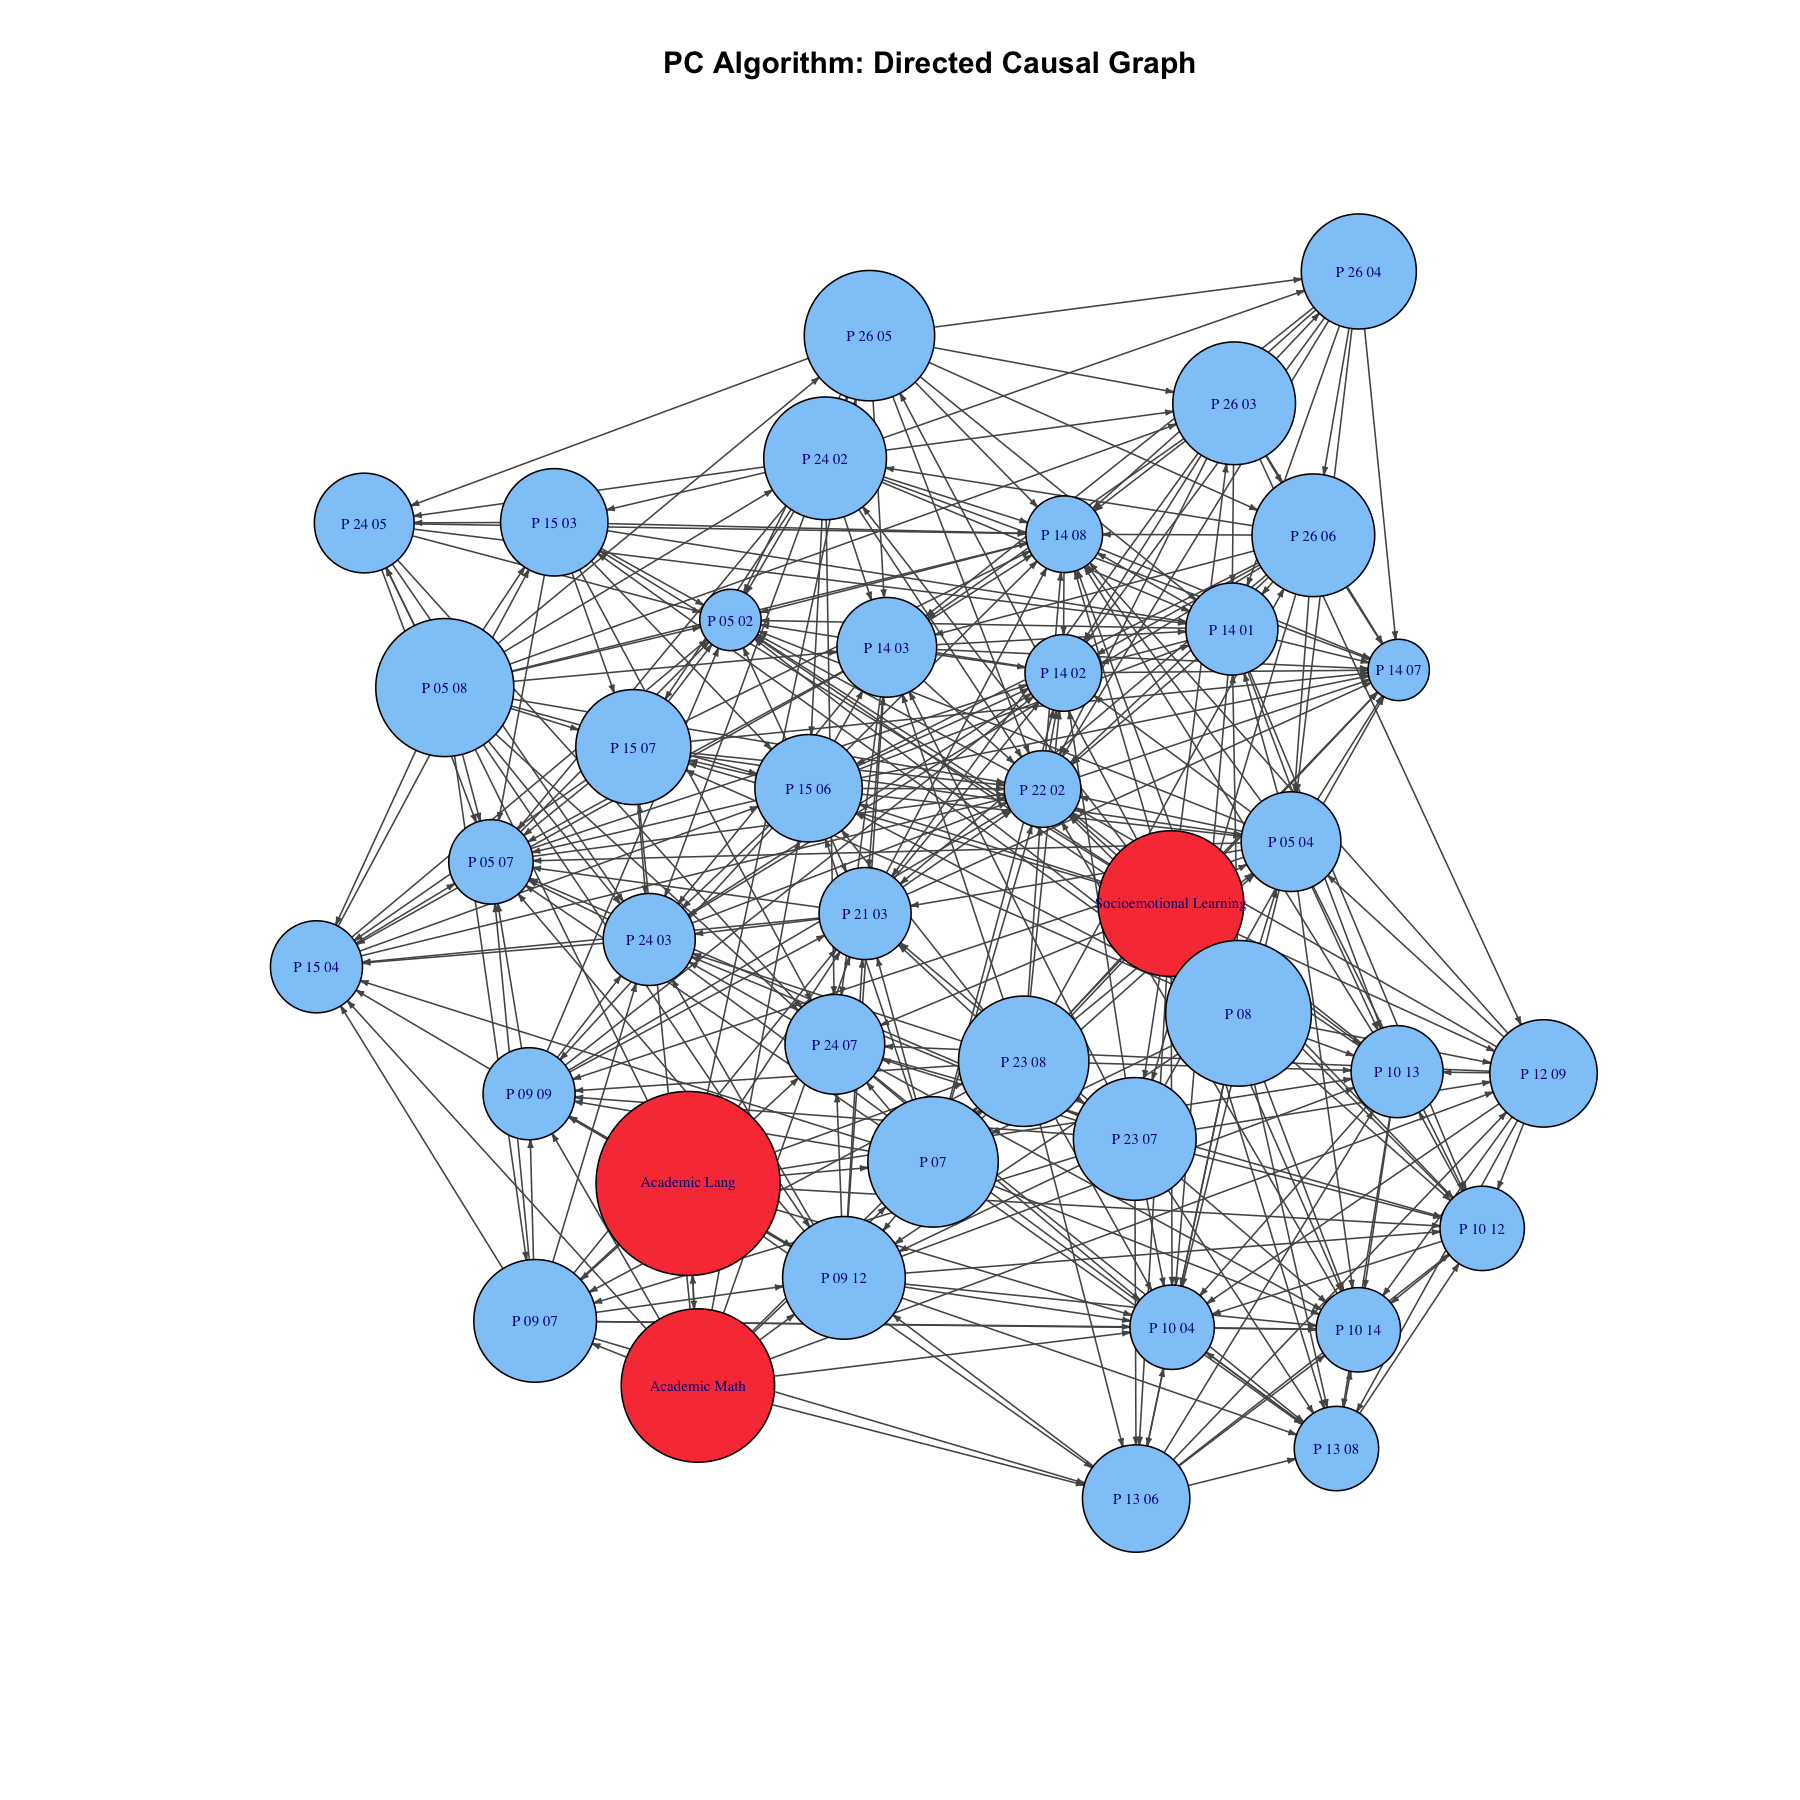
\includegraphics[width=0.98\textwidth]{pc_full_network_estudiante_questions_m4.png}
  \caption{Questions network (m=4): full graph (student questionnaire).}
\end{figure}

\begin{figure}[H]
  \centering
  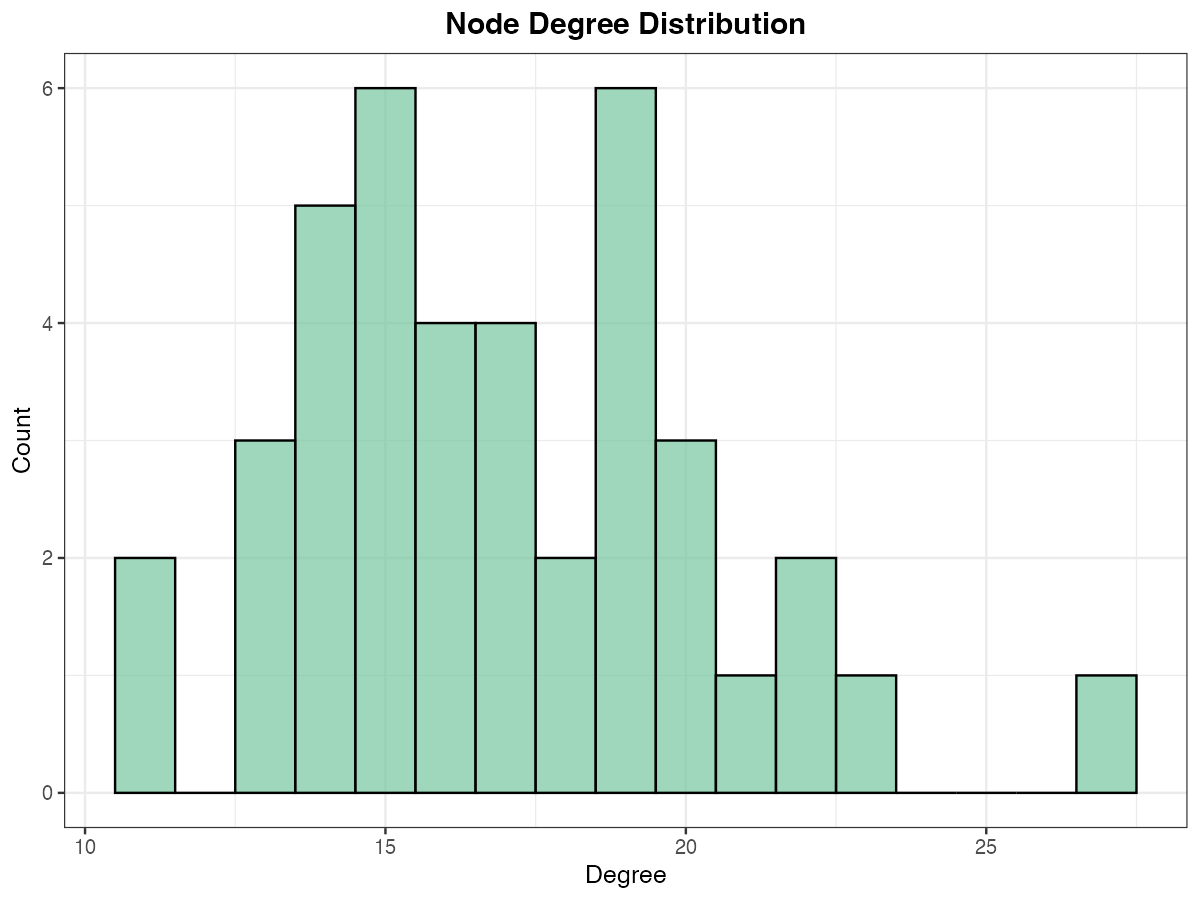
\includegraphics[width=0.7\textwidth]{pc_degree_distribution_estudiante_questions_m4.png}
  \caption{Degree distribution for the questions network (m=4).}
\end{figure}

\begin{figure}[H]
  \centering
  \begin{subfigure}[b]{0.32\textwidth}
    \centering
    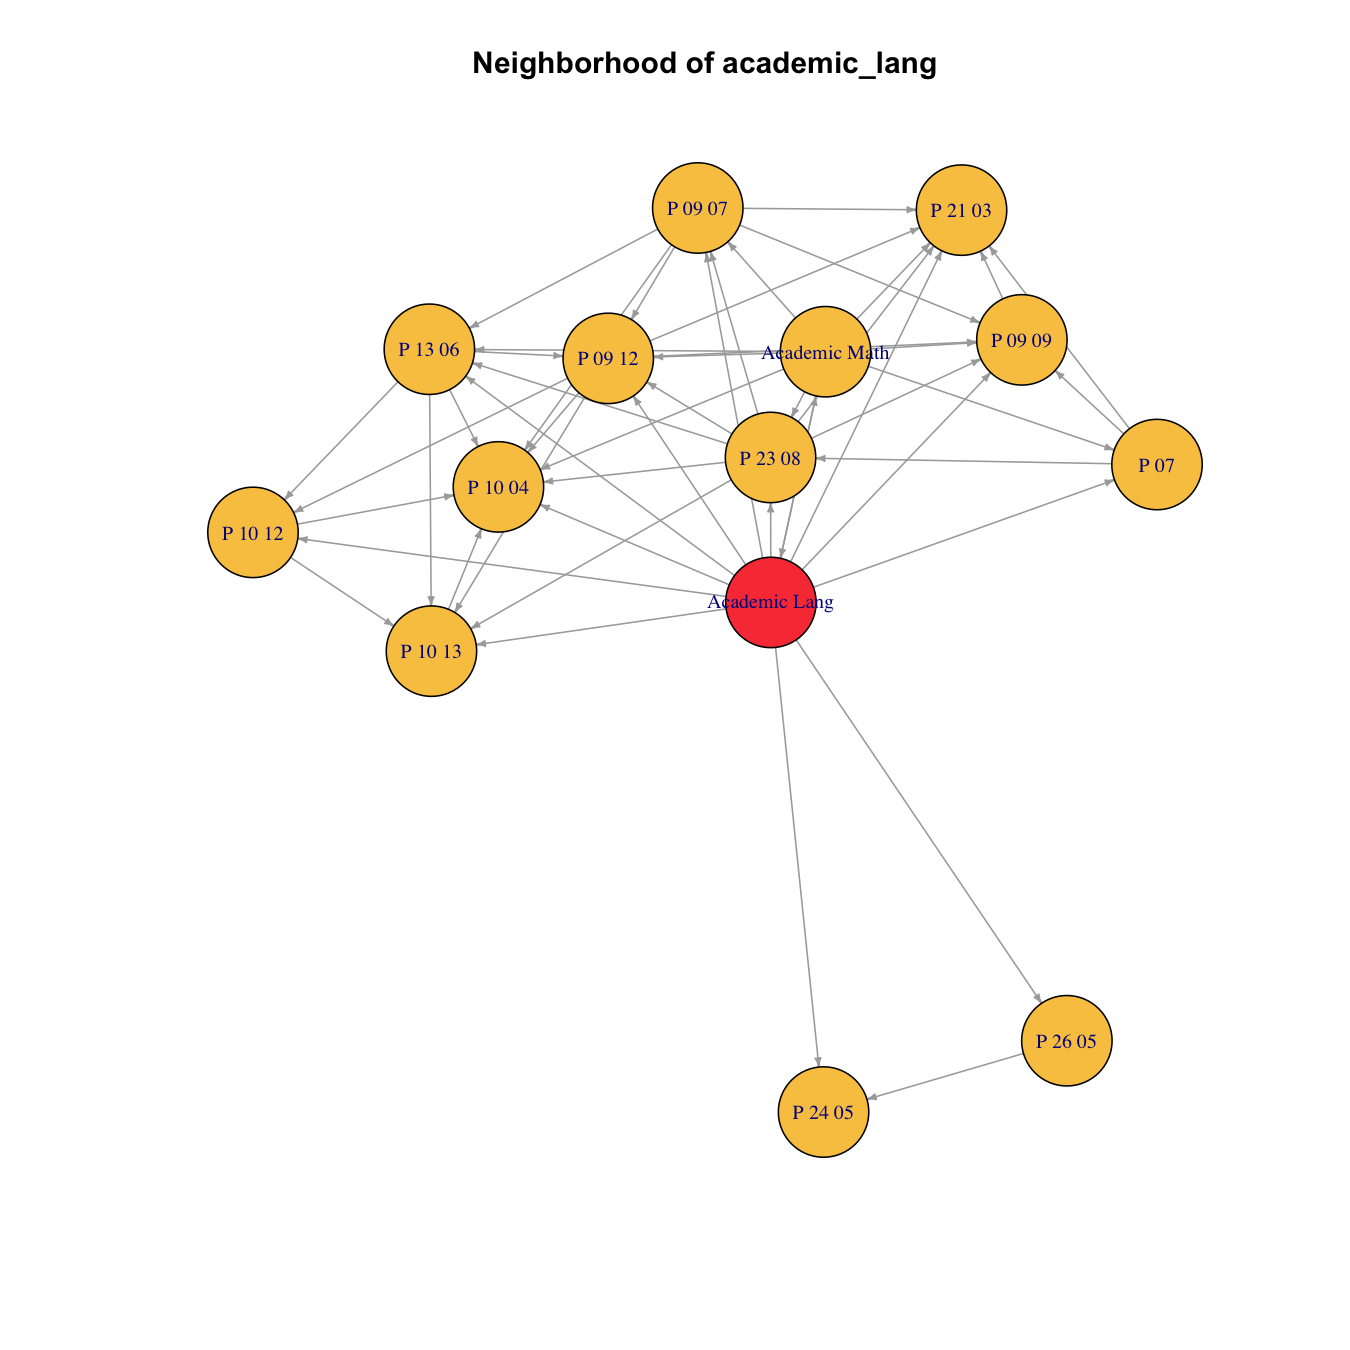
\includegraphics[width=\textwidth]{pc_estudiante_questions_academic_lang_neighborhood_m4.png}
    \caption{\texttt{academic\_lang}}
  \end{subfigure}
  \begin{subfigure}[b]{0.32\textwidth}
    \centering
    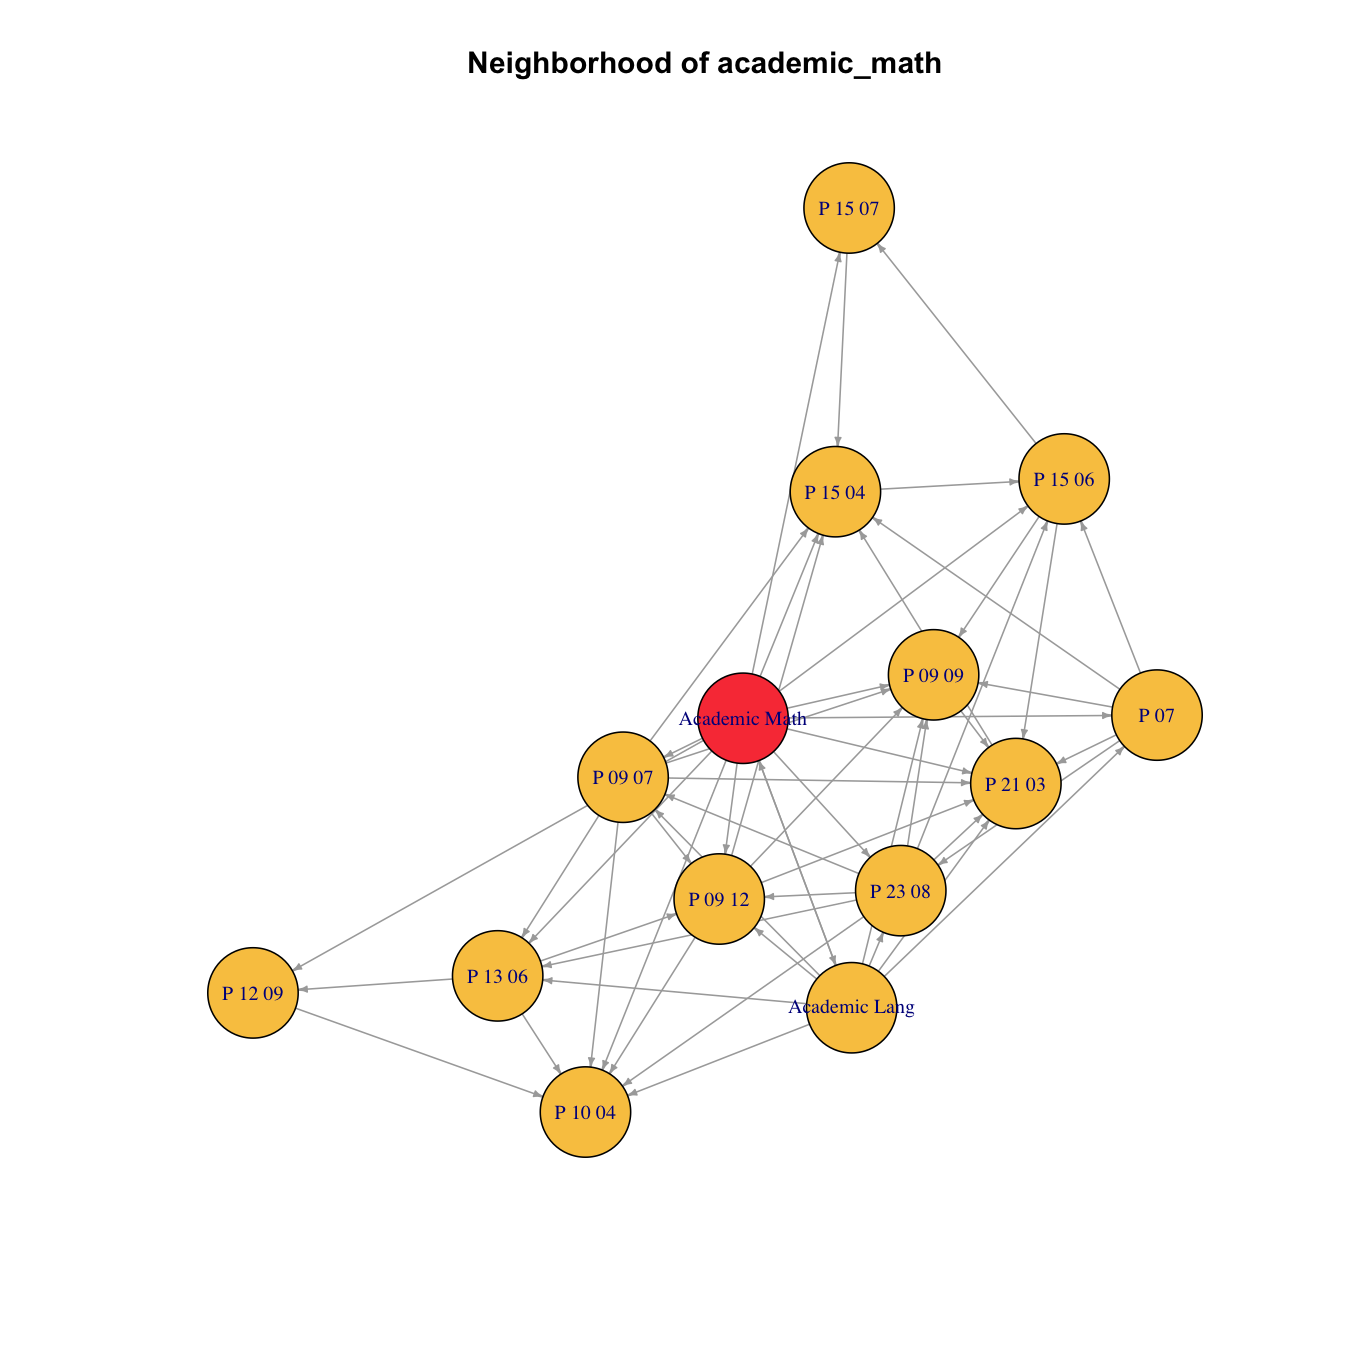
\includegraphics[width=\textwidth]{pc_estudiante_questions_academic_math_neighborhood_m4.png}
    \caption{\texttt{academic\_math}}
  \end{subfigure}
  \begin{subfigure}[b]{0.32\textwidth}
    \centering
    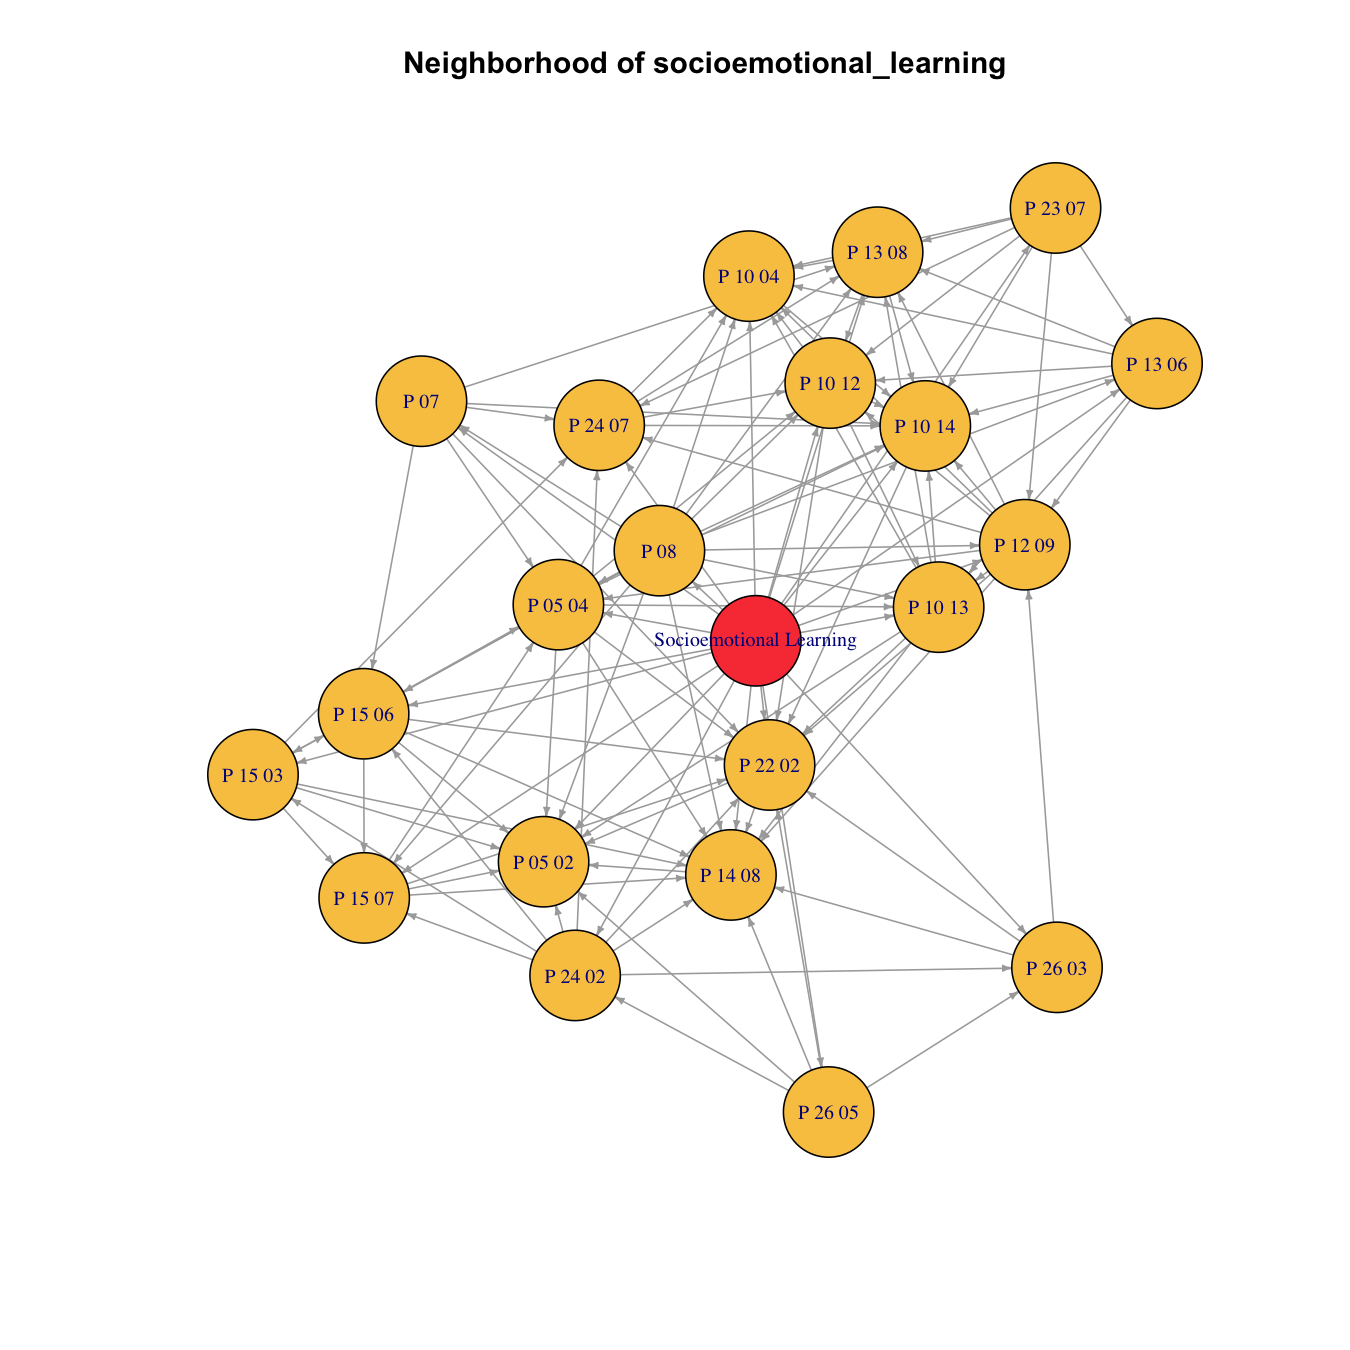
\includegraphics[width=\textwidth]{pc_estudiante_questions_socioemotional_learning_neighborhood_m4.png}
    \caption{\texttt{socioemotional\_learning}}
  \end{subfigure}
  \caption{Ego neighborhoods for the questions network (m=4).}
\end{figure}

\paragraph{Latent (m=4).}
\begin{figure}[H]
  \centering
  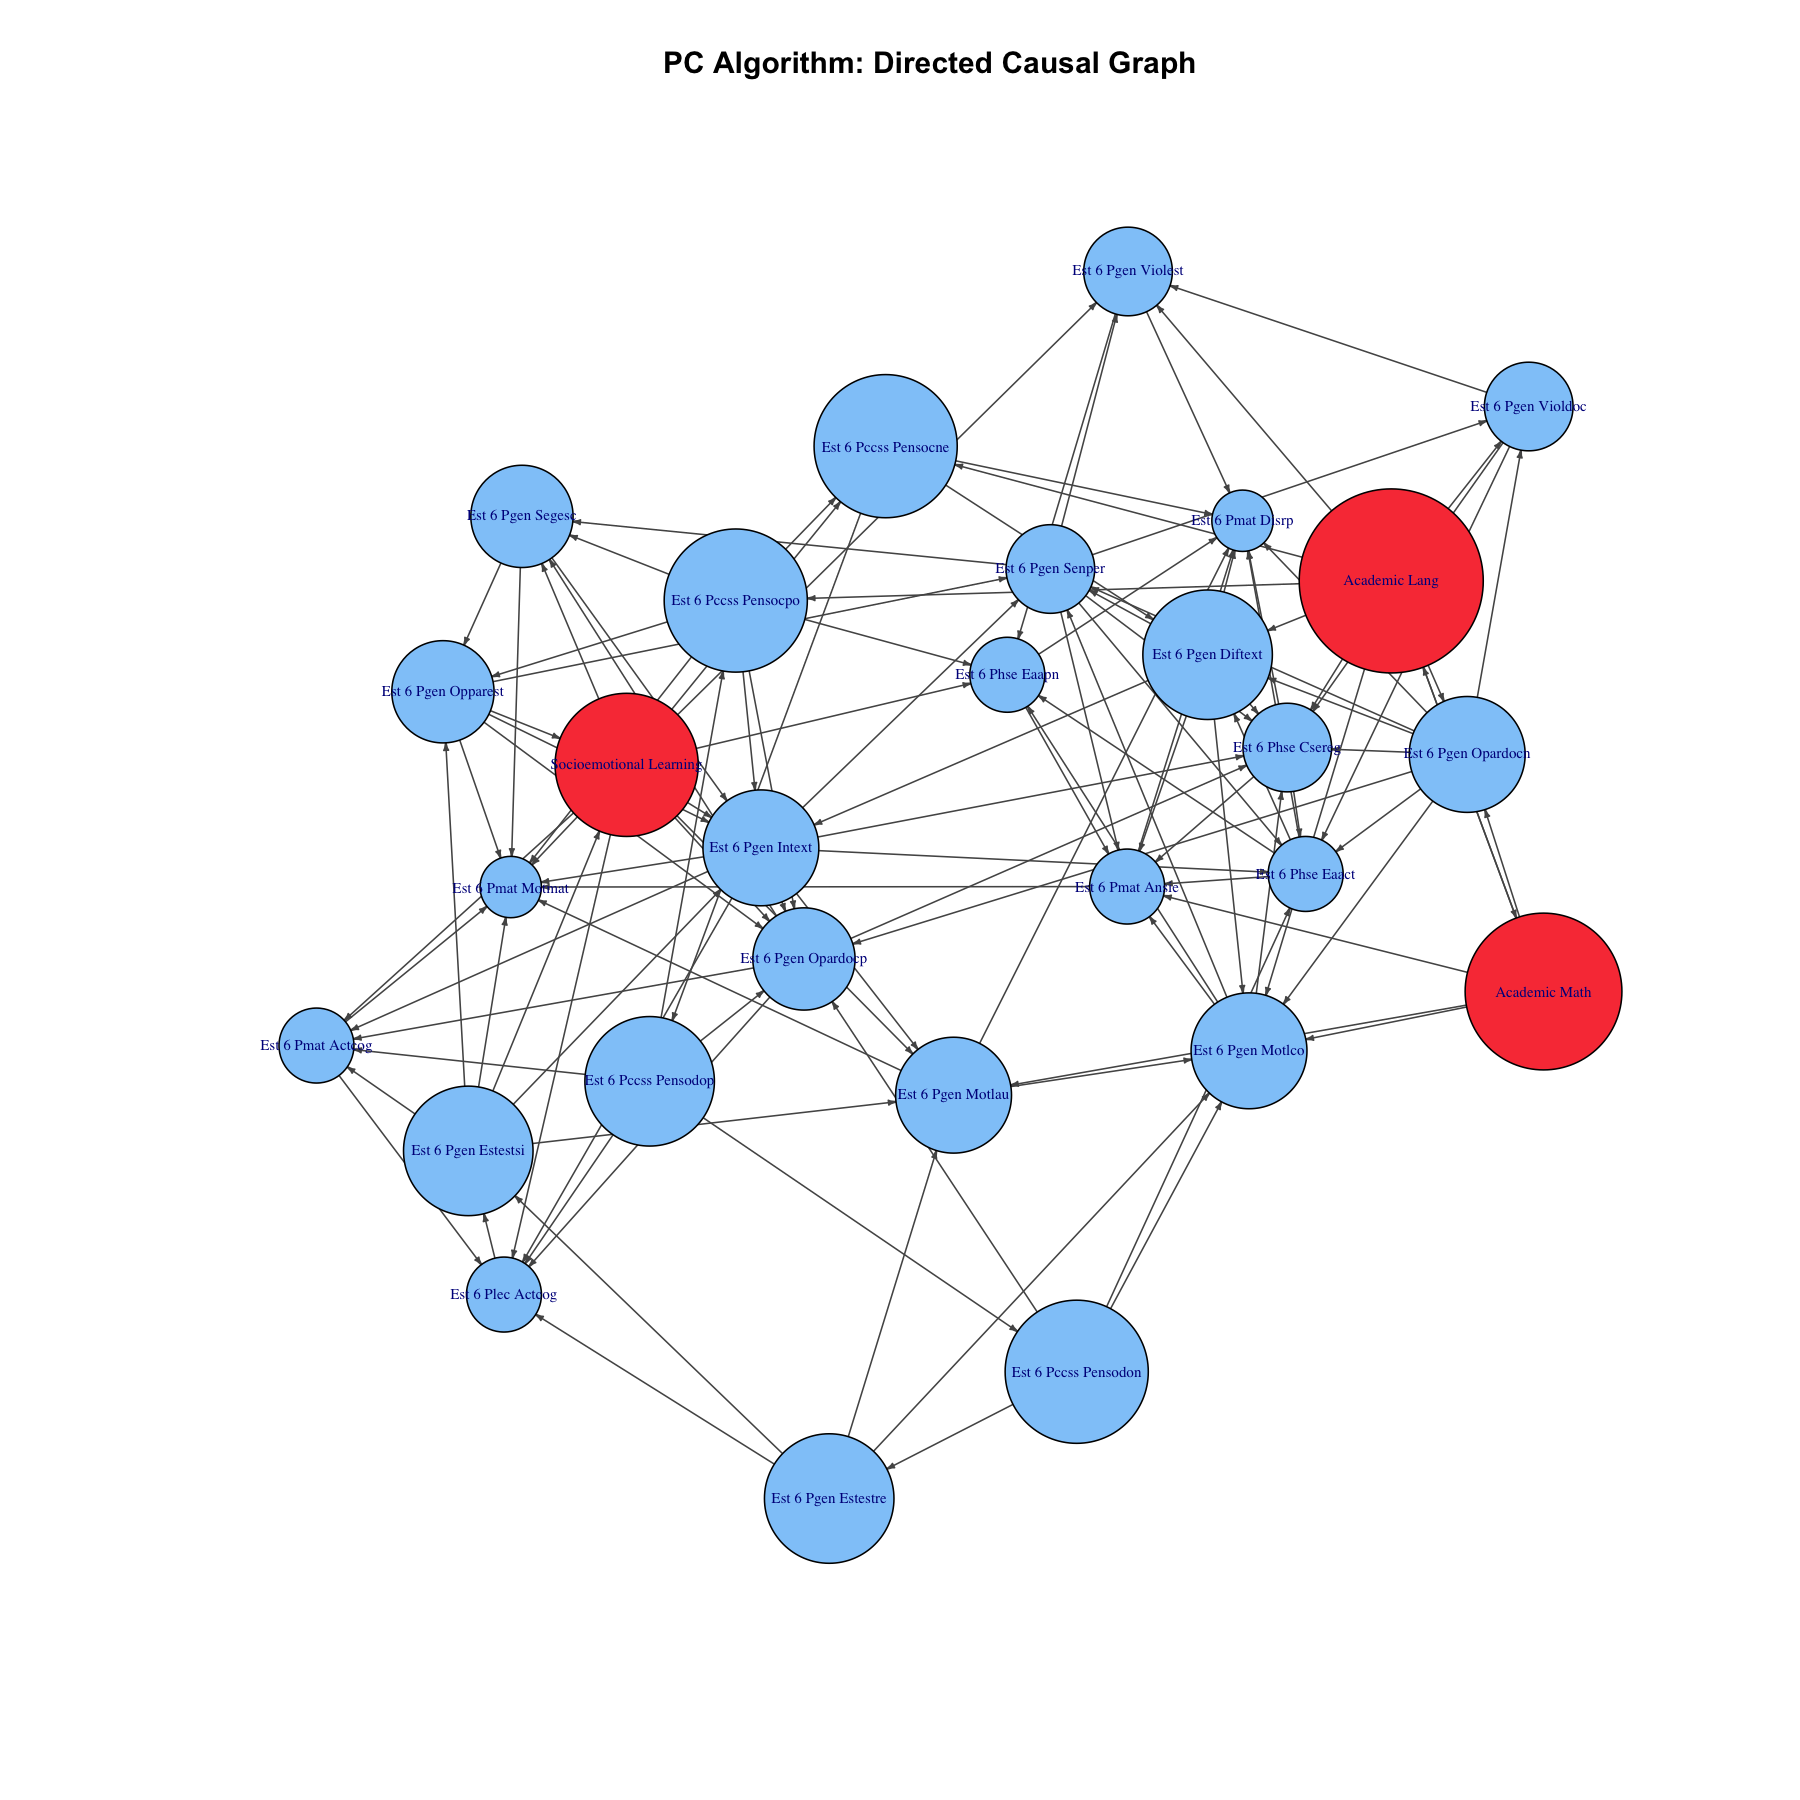
\includegraphics[width=0.98\textwidth]{pc_full_network_estudiante_latent_m4.png}
  \caption{Latent network (m=4): full graph (student questionnaire).}
\end{figure}

\begin{figure}[H]
  \centering
  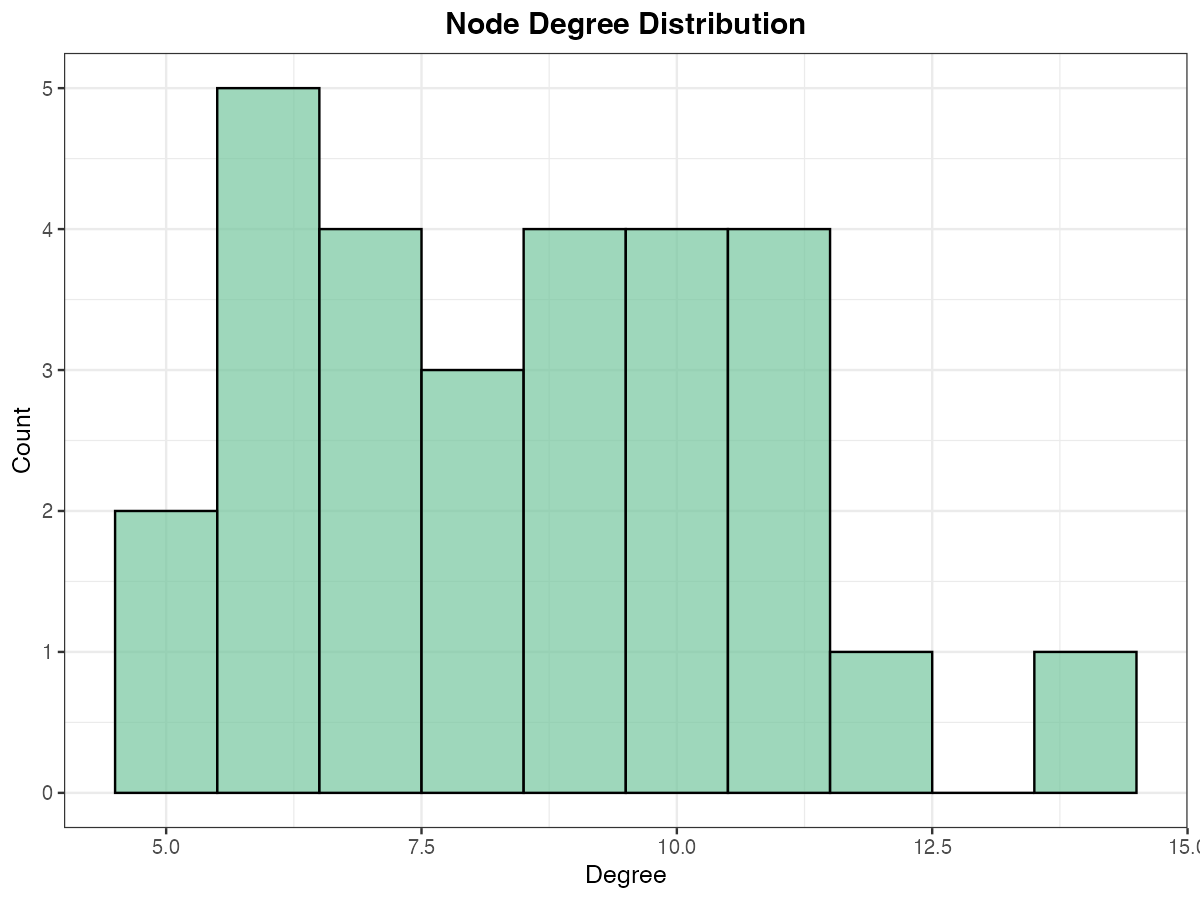
\includegraphics[width=0.7\textwidth]{pc_degree_distribution_estudiante_latent_m4.png}
  \caption{Degree distribution for the latent network (m=4).}
\end{figure}

\begin{figure}[H]
  \centering
  \begin{subfigure}[b]{0.32\textwidth}
    \centering
    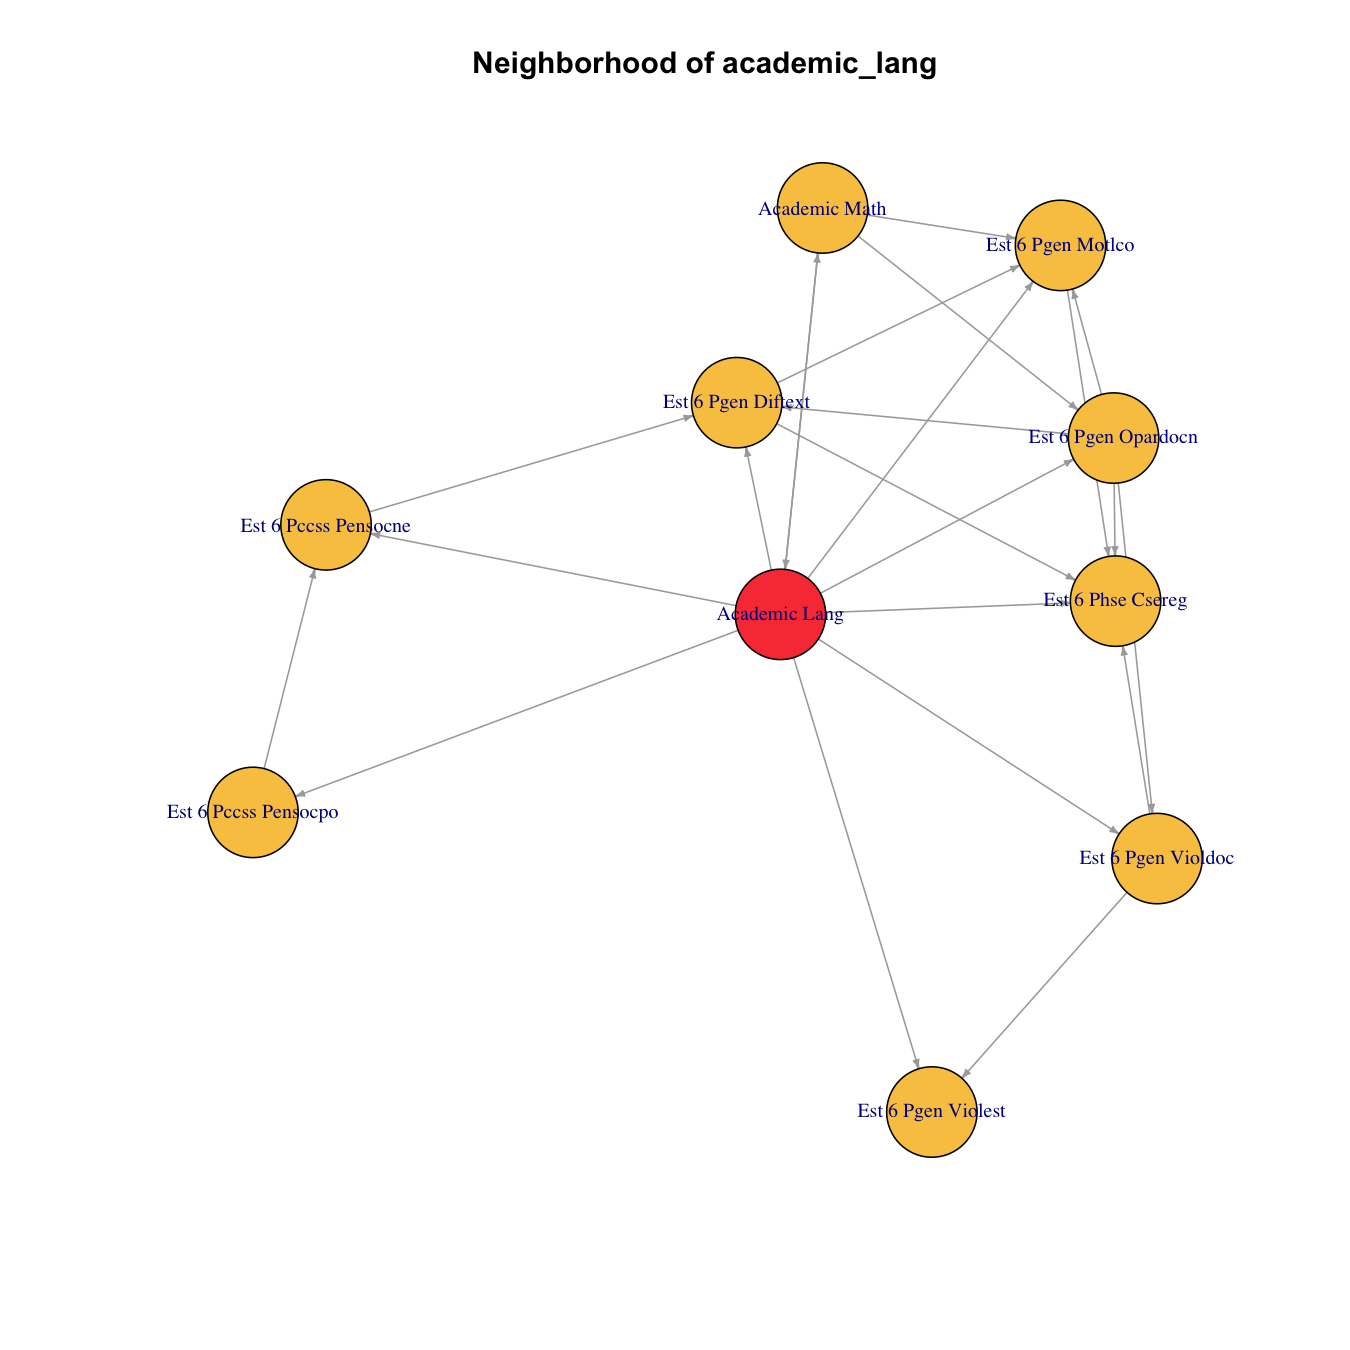
\includegraphics[width=\textwidth]{pc_estudiante_latent_academic_lang_neighborhood_m4.png}
    \caption{\texttt{academic\_lang}}
  \end{subfigure}
  \begin{subfigure}[b]{0.32\textwidth}
    \centering
    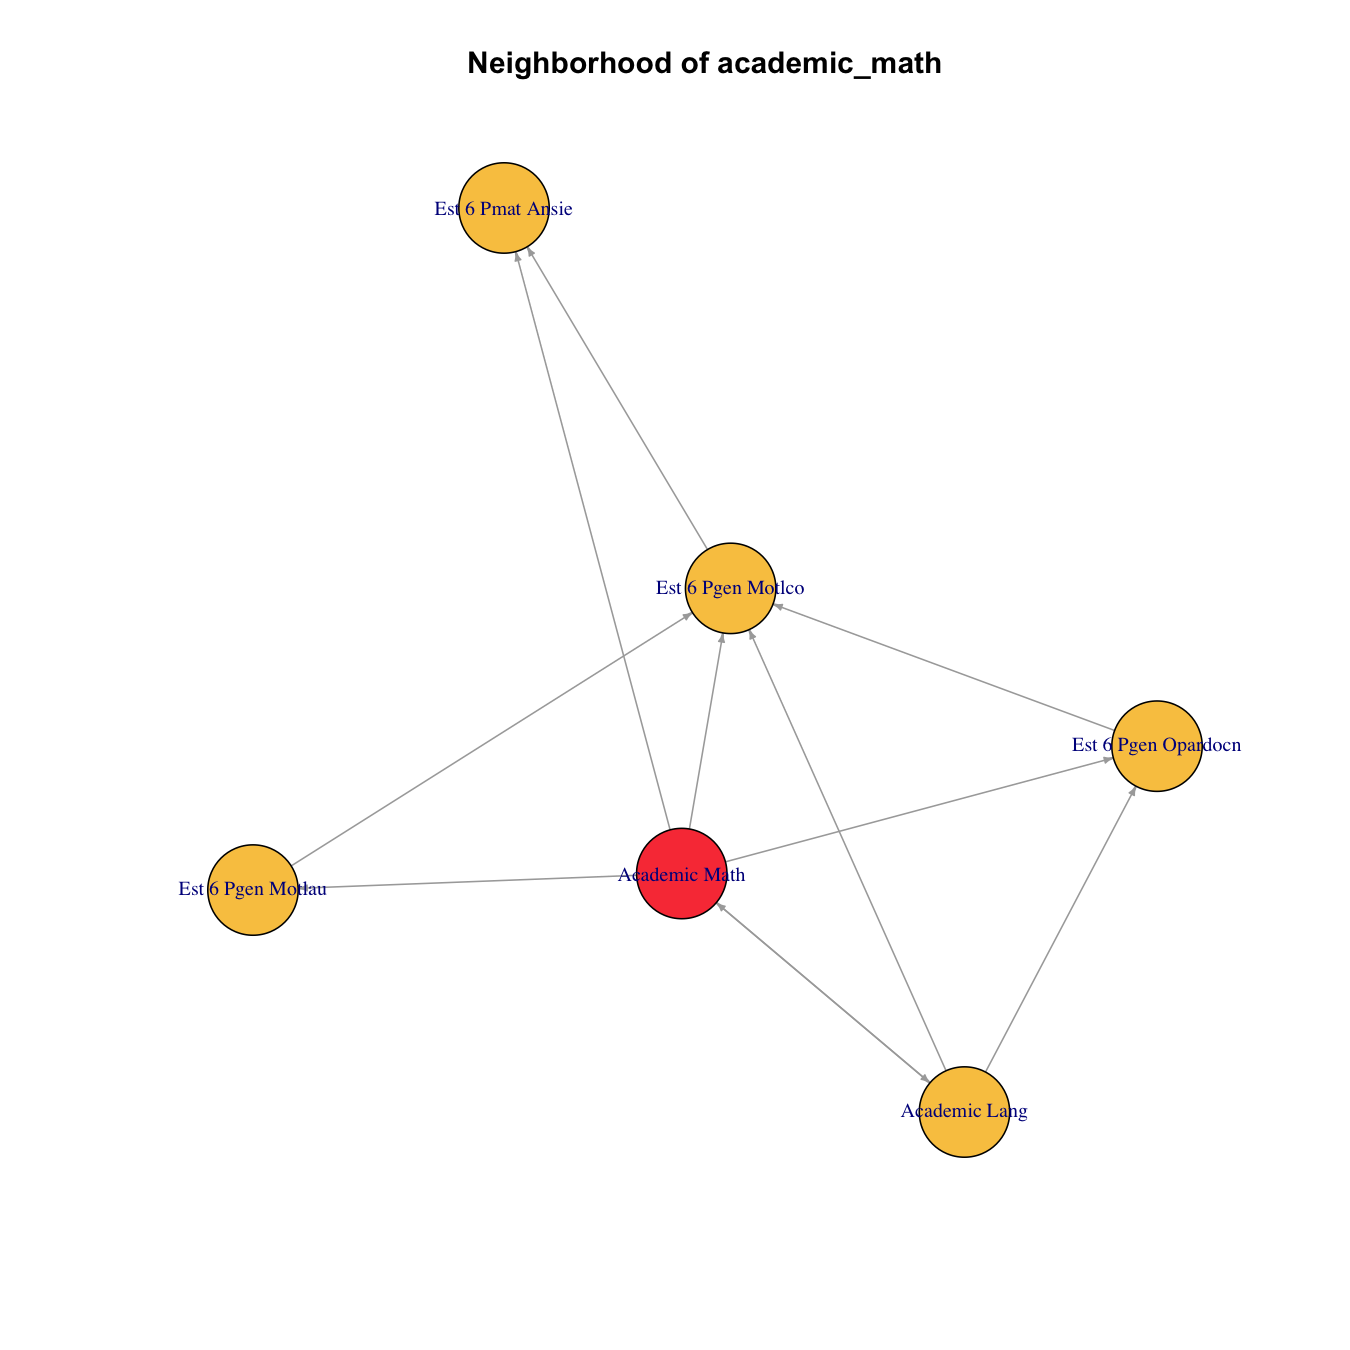
\includegraphics[width=\textwidth]{pc_estudiante_latent_academic_math_neighborhood_m4.png}
    \caption{\texttt{academic\_math}}
  \end{subfigure}
  \begin{subfigure}[b]{0.32\textwidth}
    \centering
    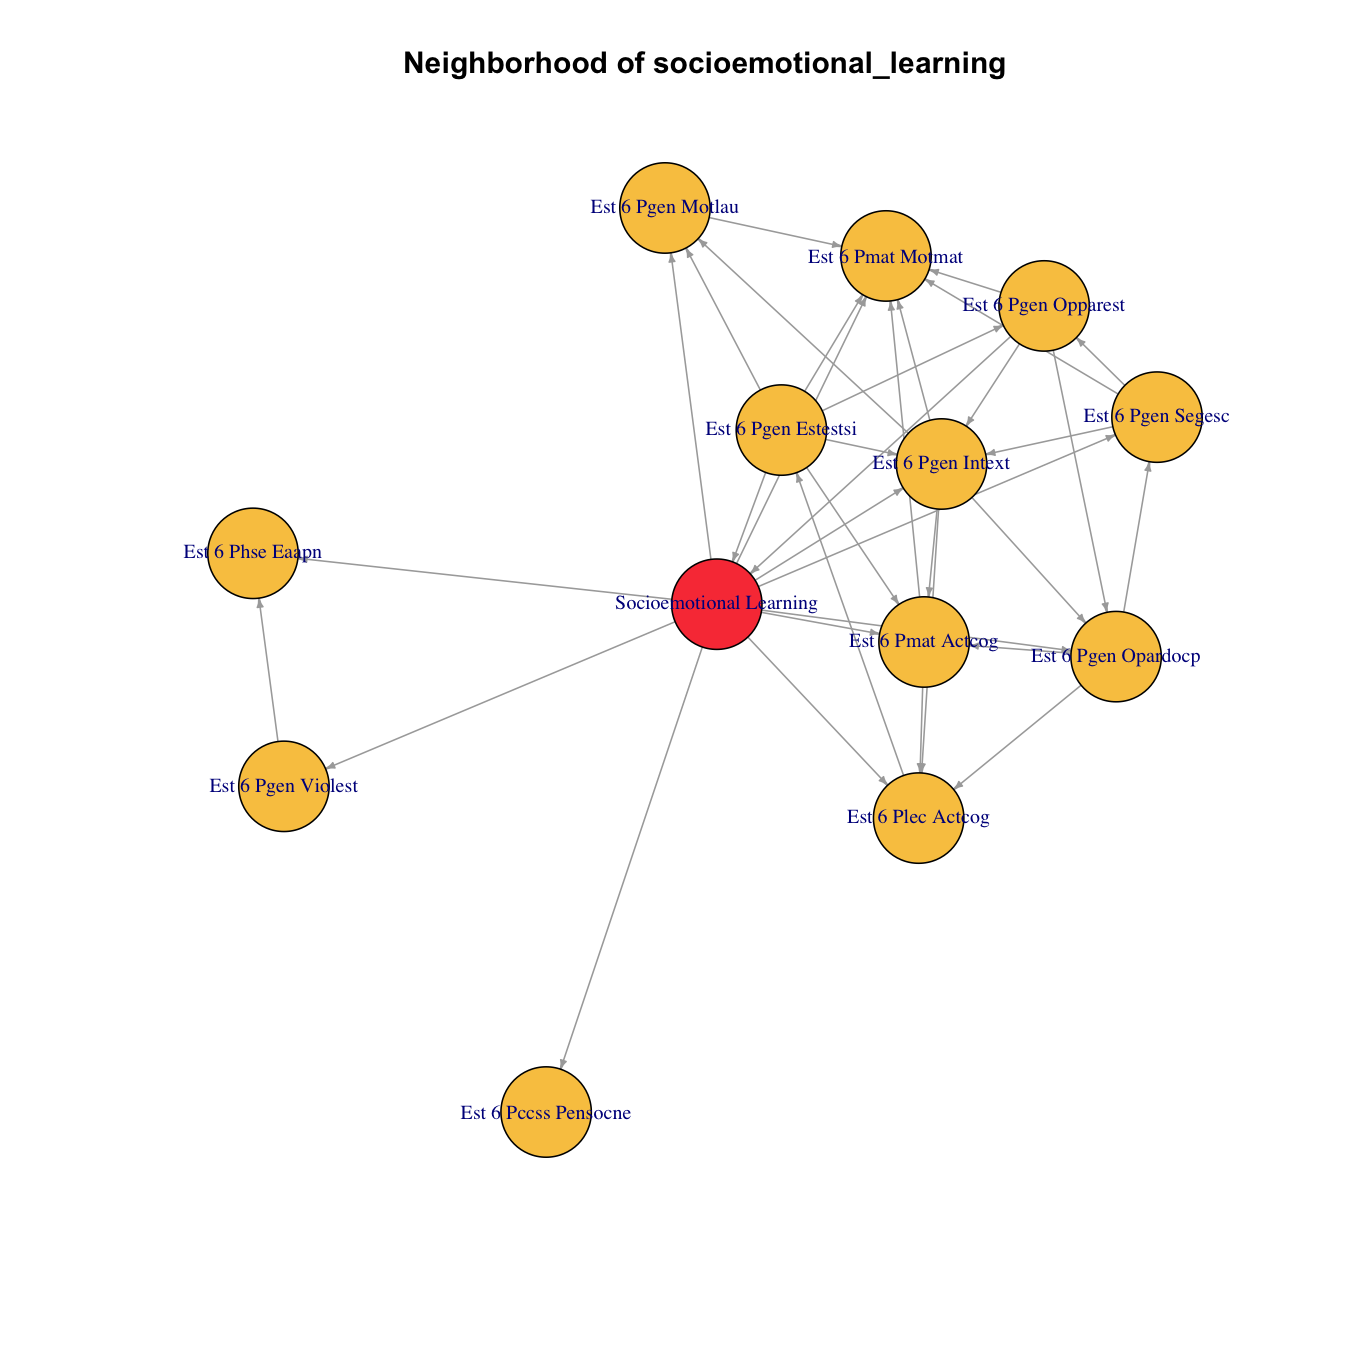
\includegraphics[width=\textwidth]{pc_estudiante_latent_socioemotional_learning_neighborhood_m4.png}
    \caption{\texttt{socioemotional\_learning}}
  \end{subfigure}
  \caption{Ego neighborhoods for the latent network (m=4).}
\end{figure}


\section{Empirical Driver Lists (Directed Parents)}
We extract directed parents for \texttt{academic\_lang}, \texttt{academic\_math}, and \texttt{socioemotional\_learning} by reading the exported edge lists and filtering for incoming arrows. Table~\ref{tab:drivers} summarizes the driver sets across networks and depths.

\begin{table}[H]
  \centering
  \caption{Directed parents (drivers) of key outcomes across networks}
  \label{tab:drivers}
  \begin{tabular}{@{}lll@{}}
    \toprule
    Network (depth) & Target & Parents \\
    \midrule
    Questions (m=3) & \texttt{academic\_lang}, \texttt{academic\_math}, \texttt{socioemotional\_learning} & (none detected) \\
    Latent (m=3) & \texttt{socioemotional\_learning} & \texttt{est6pgen\_opparest} \\
    Questions (m=4) & \texttt{academic\_lang}, \texttt{academic\_math}, \texttt{socioemotional\_learning} & (none detected) \\
    Latent (m=4) & \texttt{socioemotional\_learning} & \texttt{est6pgen\_estestsi}, \texttt{est6pgen\_opparest} \\
    \bottomrule
  \end{tabular}
\end{table}


\section{Interpretation and Recommendations}
With depth-1 conditioning, the PC algorithm favors speed and conservatism, leaving some edges undirected where the data do not support a unique orientation. Increasing \texttt{PC\_MAX\_COND\_SET} would likely resolve additional directions at the cost of runtime. In the baseline combined analysis, academic scores appear as upstream drivers of \texttt{socioemotional\_learning}; in the questionnaire-specific split, the socioemotional outcome becomes a central emitter among items, indicating the measurement scale influences graph orientation under shallow conditioning. The consistent direction from \texttt{academic\_lang} toward \texttt{academic\_math} across variants underscores a cross-domain dependency worth further study. Among latent constructs, high-degree hubs such as \texttt{EST6PGEN\_OPPAREST} act as integrators of multiple competencies and may present viable levers for targeted interventions.

\section{Reproducibility}
To regenerate these results:
\begin{enumerate}
  \item Ensure \texttt{pipeline/05\_pc\_algorithm.R} is up to date with questionnaire support.
  \item Run the script with desired environment variables, for example:
\begin{verbatim}
PC_QUESTIONNAIRE=estudiante PC_MAX_COND_SET=4 Rscript pipeline/05_pc_algorithm.R
\end{verbatim}
  \item Execute the manual network workflow (for questions and latent) as illustrated within the script to produce edges, node statistics, and figures.
\end{enumerate}

\end{document}
